\documentclass[12pt,a4paper]{scrartcl}
\newcommand{\Subchar}[2]{#1\lbrack#2\rbrack}
\usepackage{tikz}
\usetikzlibrary{positioning,snakes,decorations.text}
\usepackage{times}
\begin{document}
\begin{center}
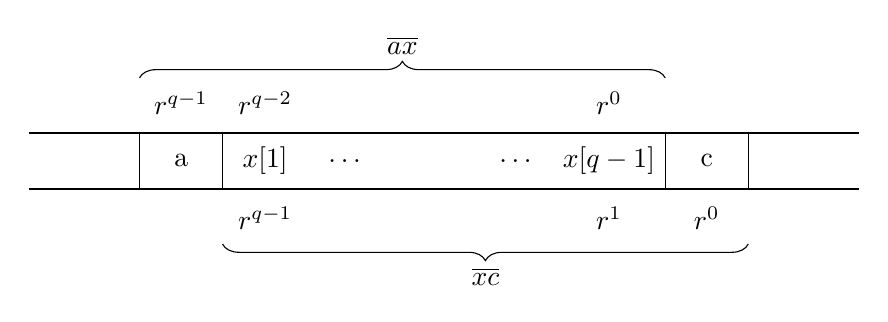
\begin{tikzpicture}
  \tikzstyle{box}=[rectangle, minimum width=30pt, minimum height=20pt]
  \foreach \x in {0,20} \draw [thick] (0,\x pt) -- +(300pt,0);
  % left nodes
  \draw (55pt,10pt) node (a) [draw, box] {a}
    node (x1) [box, right=0pt of a] {$\Subchar{x}{1}$}
    node [above=3pt of a] {$r^{q-1}$}
    node [above=3pt of x1] {$r^{q-2}$}
    node [below=3pt of x1] {$r^{q-1}$}
    node [box, right=0 of x1] {$\ldots~$};
  % right nodes
  \draw (245pt,10pt) node (c) [draw, box] {c}
    node (x2) [box,left=0pt of c] {$\Subchar{x}{q-1}$}
    node [below=3pt of c] {$r^0$}
    node [below=3pt of x2] {$r^1$}
    node [above=3pt of x2] {$r^0$}
    node [box, left=0 of x2] {$~\ldots$};
  % braces
  \draw [decorate, decoration={brace, mirror, amplitude=6pt}] (70pt,-20pt) -- +(190pt,0)
    node [pos=0.5, below=5pt] {$\overline{xc}$};
  \draw [decorate, decoration={brace, amplitude=6pt}] (40pt,40pt) -- +(190pt,0)
    node [pos=0.5, above=5pt] {$\overline{ax}$};
\end{tikzpicture}
\end{center}
\end{document}
